
%%% Local Variables: 
%%% mode: latex
%%% TeX-master: "lista1"
%%% End: 
\documentclass[11pt,epsf]{report}
\setlength{\vsize}{297mm}
\setlength{\hsize}{210mm}
\setlength{\textheight}{230mm}
\setlength{\textwidth}{170mm}
%\voffset -2.5cm
\hoffset -2.5cm

\usepackage[latin1]{inputenc}
%\usepackage{latexsym}
%\usepackage{amssymb}
\usepackage[dvips]{graphicx}

\newenvironment{alternativas}{\renewcommand{\labelenumi}{(\alph{enumi})}\begin{enumerate}\addtolength{\itemsep}{-2.5mm}\setlength{\parsep}{0pt}}{\end{enumerate}}

\newcounter{qcounter}
\newenvironment{question}{\stepcounter{qcounter}\paragraph{\arabic{qcounter}.}}{}




\begin{document}

\begin{center}
ENG04035 - Sistemas de Controle I \\
 Prof. Jo�oo Manoel Gomes da Silva Jr. e Romeu Reginatto \\
Resposta Transit�ria e Identifica��o de Par�metros de Fun��es de Transfer�ncia
\end{center}


\begin{question}
Ler o cap�tulo 4, p�ginas 123 a 178, "Resposta no Dom�nio do Tempo",
do livro: N. S. Nise, {\em Engenharia de Sistemas de Controle}, dispon�vel 
no xer�x (as se��es 4.9 a 4.11 n�o ser�o necess�rias neste momento). 

 Em seguida, resolver os seguintes problemas propostos no livro 
(in�cio na pag. 170): 2, 4, 6, 8, 17, 19, 20, 23, 24, 29, 
{\em 30}, 49, 50, {\em 58}, 61. Os problemas considerados avan�ados 
foram aqui marcados em it�lico.
\end{question}


\begin{question}
A figura abaixo ilustra a resposta ao degrau unit�rio de 3 sistemas
distintos. Obtenha um modelo aproximado para cada um deles, em
termos de uma fun��o de transfer�ncia.
\begin{center}
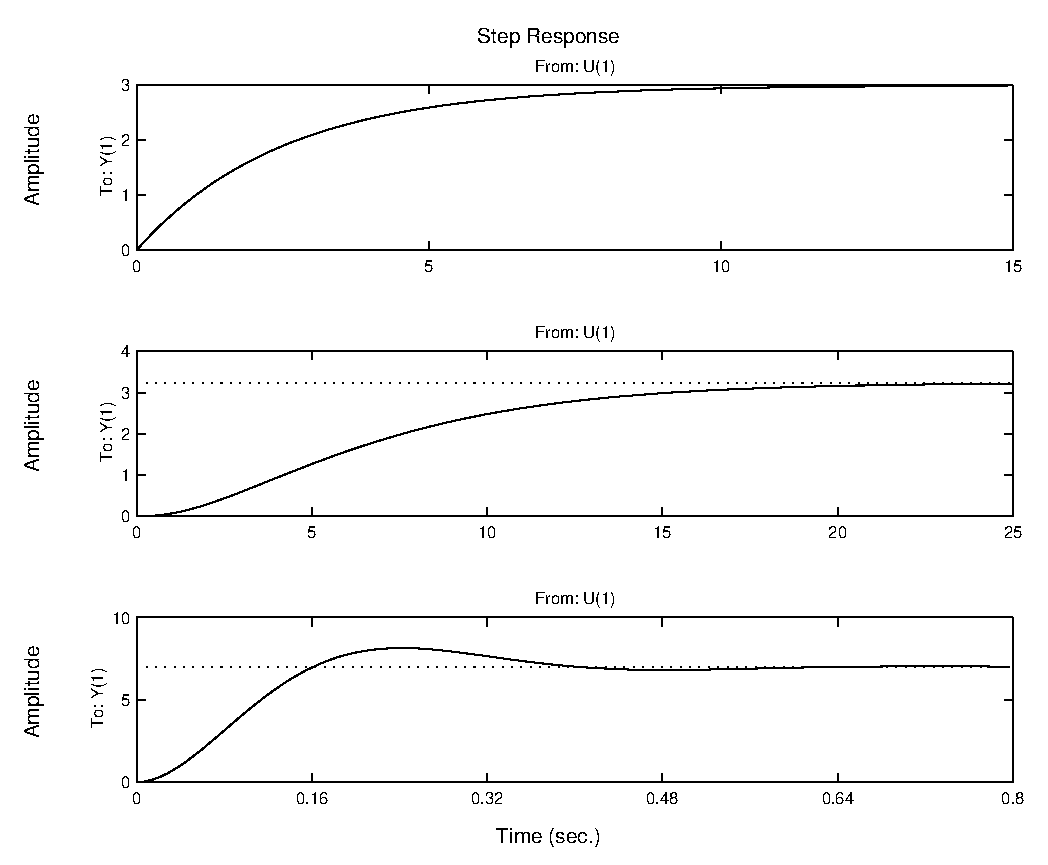
\includegraphics[width=17cm,height=16cm]{identfig1.eps}
\end{center}

\end{question}


\end{document}











